\documentclass[chi_draft]{sigchi}

% Use this section to set the ACM copyright statement (e.g. for
% preprints).  Consult the conference website for the camera-ready
% copyright statement.

% Copyright
%\CopyrightYear{2016}
%\setcopyright{acmcopyright}
%\setcopyright{acmlicensed}
%\setcopyright{rightsretained}
%\setcopyright{usgov}
%\setcopyright{usgovmixed}
%\setcopyright{cagov}
%\setcopyright{cagovmixed}
% DOI
%\doi{http://dx.doi.org/10.475/123_4}
% ISBN
%\isbn{123-4567-24-567/08/06}
%Conference
%\conferenceinfo{CHI'16,}{May 07--12, 2016, San Jose, CA, USA}
%Price
%\acmPrice{\$15.00}

% Use this command to override the default ACM copyright statement
% (e.g. for preprints).  Consult the conference website for the
% camera-ready copyright statement.

%% HOW TO OVERRIDE THE DEFAULT COPYRIGHT STRIP --
%% Please note you need to make sure the copy for your specific
%% license is used here!
\toappear{
% Permission to make digital or hard copies of all or part of this work
% for personal or classroom use is granted without fee provided that
% copies are not made or distributed for profit or commercial advantage
% and that copies bear this notice and the full citation on the first
% page. Copyrights for components of this work owned by others than ACM
% must be honored. Abstracting with credit is permitted. To copy
% otherwise, or republish, to post on servers or to redistribute to
% lists, requires prior specific permission and/or a fee. Request
% permissions from \href{mailto:Permissions@acm.org}{Permissions@acm.org}. \\
% \emph{CHI '16},  May 07--12, 2016, San Jose, CA, USA \\
% ACM xxx-x-xxxx-xxxx-x/xx/xx\ldots \$15.00 \\
% DOI: \url{http://dx.doi.org/xx.xxxx/xxxxxxx.xxxxxxx}
}

% Arabic page numbers for submission.  Remove this line to eliminate
% page numbers for the camera ready copy
% \pagenumbering{arabic}

% Load basic packages
\usepackage{balance}       % to better equalize the last page
\usepackage{graphics}      % for EPS, load graphicx instead 
\usepackage[T1]{fontenc}   % for umlauts and other diaeresis
\usepackage{txfonts}
\usepackage{mathptmx}
\usepackage[pdflang={en-US},pdftex]{hyperref}
\usepackage{color}
\usepackage{booktabs}
\usepackage{textcomp}

% Some optional stuff you might like/need.
\usepackage{microtype}        % Improved Tracking and Kerning
% \usepackage[all]{hypcap}    % Fixes bug in hyperref caption linking
\usepackage{ccicons}          % Cite your images correctly!
% \usepackage[utf8]{inputenc} % for a UTF8 editor only

% If you want to use todo notes, marginpars etc. during creation of
% your draft document, you have to enable the "chi_draft" option for
% the document class. To do this, change the very first line to:
% "\documentclass[chi_draft]{sigchi}". You can then place todo notes
% by using the "\todo{...}"  command. Make sure to disable the draft
% option again before submitting your final document.
\usepackage{todonotes}
\usepackage{paralist}
\usepackage{lscape}
\usepackage{url}

% Paper metadata (use plain text, for PDF inclusion and later
% re-using, if desired).  Use \emtpyauthor when submitting for review
% so you remain anonymous.
\def\plaintitle{Clash of Crowds: Understanding Human \\ Text Classification though Crowdsourcing Games}
\def\plainauthor{First Author, Second Author, Third Author,
  Fourth Author, Fifth Author, Sixth Author}
\def\emptyauthor{}
\def\plainkeywords{Authors' choice; of terms; separated; by
  semicolons; include commas, within terms only; required.}
\def\plaingeneralterms{Documentation, Standardization}

% llt: Define a global style for URLs, rather that the default one
\makeatletter
\def\url@leostyle{%
  \@ifundefined{selectfont}{
    \def\UrlFont{\sf}
  }{
    \def\UrlFont{\small\bf\ttfamily}
  }}
\makeatother
\urlstyle{leo}

% To make various LaTeX processors do the right thing with page size.
\def\pprw{8.5in}
\def\pprh{11in}
\special{papersize=\pprw,\pprh}
\setlength{\paperwidth}{\pprw}
\setlength{\paperheight}{\pprh}
\setlength{\pdfpagewidth}{\pprw}
\setlength{\pdfpageheight}{\pprh}

\newcommand{\tabincell}[2]{\begin{tabular}{@{}#1@{}}#2\end{tabular}}
\usepackage{paralist}
\newcommand{\pro}[1]{\text{#1}}
\newcommand{\con}[1]{\text{#1}}

% Make sure hyperref comes last of your loaded packages, to give it a
% fighting chance of not being over-written, since its job is to
% redefine many LaTeX commands.
\definecolor{linkColor}{RGB}{6,125,233}
\hypersetup{%
  pdftitle={\plaintitle},
% Use \plainauthor for final version.
%  pdfauthor={\plainauthor},
  pdfauthor={\emptyauthor},
  pdfkeywords={\plainkeywords},
  pdfdisplaydoctitle=true, % For Accessibility
  bookmarksnumbered,
  pdfstartview={FitH},
  colorlinks,
  citecolor=black,
  filecolor=black,
  linkcolor=black,
  urlcolor=linkColor,
  breaklinks=true,
  hypertexnames=false
}

% create a shortcut to typeset table headings
% \newcommand\tabhead[1]{\small\textbf{#1}}

% End of preamble. Here it comes the document.
\begin{document}

\title{\plaintitle}

\numberofauthors{1}
\author{%
  \alignauthor{Tongshuang Wu \quad Jim Chen \quad Chenglong Wang\\
    \affaddr{University of Washington, USA}\\
    \email{\textsf{\{wtshuang, cqz, clwang\}@cs.washington.edu}}
    }\\
}

\maketitle

\begin{abstract}
Human assisted feature extraction and selection is becoming popular in the field of interactive Machine Learning (iML). Prior work commonly builds on assumptions that human involvement contributes positively without attempting to understand how humans interpret the features being used. In this work, we attempt to form a better understanding of human feature extraction process by indirectly learning and verifying latent features humans are using through gamifying the simultaneous labeling and feature selection procedure.

We designed and compared four interactive games against a baseline implementation of a common feature optimization system and between each other on text sentiment labeling task. Through our experiments, we attempt to map human judgment onto a model using a constrained feature set (bag-of-words model) to learn if and how human judgments may effectively inform machine learning models.
\end{abstract}

%\category{H.5.m.}{Information Interfaces and Presentation
%  (e.g. HCI)}{Miscellaneous} \category{See
%  \url{http://acm.org/about/class/1998/} for the full list of ACM
%  classifiers. This section is required.}{}{}

%\keywords{\plainkeywords}

\section{Introduction}

Interactive feature selection has become mainstream in interactive Machine Learning (iML).
Current classification systems have been taking advantage of human judgments to select predictive features to build effective machine learning models~\cite{brooks2015featureinsight, cheng2015flock}. 
For instance, FeatureInsight~\cite{brooks2015featureinsight} presents an interactive feature selection system that allows humans to select word features that will assist text classification tasks.

While general belief in the past was that humans could contribute their domain knowledge to the models~\cite{stumpf2009interacting}, new studies have shown that human intersections are not as effective as we have hoped. Even worse, some of these interactive approaches even see decreased performance on multiple models~\cite{fiebrink2011human,stumpf2009interacting}.
A potential barrier for designers of iML systems is how to make good use of interactive approaches with the limited knowledge on modelling humans input effectiveness.

There are a few reasons that direct application of human judgement may result in suboptimal outcomes: 

Firstly, current feature selection procedures may not reflect underlying reasoning structures feature engineers are actually using.
Prior work (e.g.,~\cite{trivedi2015interactive}) has been done to understand features that human use by mapping users' mental model into concrete words in the document. The approach used to collect such features (i.e., ``human features''), take sentiment analysis for example, is to directly ask users to (1) label a document and (2) then select words associated with this decision it. 

While such techniques are straightforward, it is unclear whether features collected in this way suffer from the ``hindsight bias'' effect of human labelers. 
In fact, Gazzaniga et al.~\cite{gazzaniga2013integrated} has shown that people are generally poor at introspecting on the signals they use to make decisions. In other words, post-hoc word selection could lead users to ``make up'' reasons (i.e., words) that they believe best explain their completed labeling decision, rather than the ones that reflect their instincts (or ones they used in the decision making process). If such an effect exists, labels and features collected from existing approaches are not guaranteed to be naturally paired. Additionally, diverging understanding of the task may also result in different features being selected among human workers.

Second, we have not yet understood whether computers and humans proceed a classification task in the same way. Most state-of-art iML systems use linear models like Naive Bayes~\cite{kulesza2015principles, kulesza2011oriented, amershi2012regroup} as their underlying classification model because of its interpretability.
Such algorithms are well known for making use of the bag-of-words models such as frequencies of n-grams for text classification. On the other hand, it is unclear whether humans make their judgments with a similar model, and directly combining humans' decision making model (which produces features) with the model using in automated training is questionably beneficial. With model discrepancies in mind, human-chosen features could be different from, and potentially not transferable to existing machine learning models.

As a result of the observations above, understanding human understanding in feature selection (or human decision making) is crucial for building effective iML systems. Instead of simply providing features that humans identify from an arbitrary personal measures and iterating through a tedious ``trial-and-error'' procedure, our work seeks to understand the distinction between ``what humans can provide'' and ``what computers can intake'' by comparing and articulating the differences between the classification process of humans and computers. Such understanding could guide humans to effectively contribute their domain knowledge in a way that the machines can use. In this paper, we ground our experiment on sentiment analysis tasks, which is among most important and fundamental classification tasks and is intuitive enough so that human understanding will not obstruct our learning.

Concretely, we aim to explore two things in our experiment: (1) how do human understanding for document sentiment map onto unigram bag-of-words features, and (2) whether we can effectively extract real ``human features'', or the understanding-word mappings as mentioned, through certain workflow designs.

To achieve this, we transform the feature extraction workflow into four different games, namely the collaborative games \emph{Bingo} and \emph{Hangman-add}, and the competitive ones \emph{Hangman-subtract} and \emph{Censor}.
All the games support simultaneous collections of document labels and features to ensure feature-label mapping.
By manipulating the users' possible inputs and their access to information in each game, we try to indirectly learn and verify latent features humans actually use. 

Deploying the games to Amazon Mechanical Turk (AMT), we examine how our games may support effective elicitation of various sets of human features (e.g., minimal set for facilitating decision making, inclusive superset of features will allow human classifiability). 
% and evaluate the how different incentives affect participants' feature extraction. 
% --- We don't do this (See Proposal!)

Through our experiments and analysis we come to the conclusion \todo{Summarize the analysis result when done.}

Our contributions are as follows:
\begin{compactitem}
	\item Proposal of a new game-based approach for both \emph{collecting} and \emph{verifying} features used by human in sentiment labeling tasks.
  \item Implementation and deployment of games to collect users game statistics, from which we learned a few principles of human features that can be used to aid iML system design.
  \item \todo{more?} 
\end{compactitem}


%In order to design interactive machine learning systems that better coordinate human and computer, system designers need to have a good understanding on how human and computer make their decisions \todo{add some citation to justify this}. For example, in order to design a interactive machine learning system for text sentiment classification, one needs to know which words in the text are features used by humans and computers to make their decisions (whether a document is positive or negative). While features used by machine learning algorithms, e.g., n-gram model, are well understood, little is know about what are the text features used by human in their decision making process. Our project seeks to understand the human labeling process (the connection between labels created by human and feature words influence them most in the labeling process) in the context of \emph{text sentiment labeling tasks}. 


%In order to collect more meaningful features and provides better explanation of the these features, our key insight is to collect features along with labels during the labeling procedure though interactive games. Concretely, we designed a set of 5 crowd sourcing games: \emph{DirectAnnotation}, \emph{Bingo}, \emph{HangmanAdd}, \emph{HangmanSub} and \emph{Censor}. While these games share the same goal, players in different games have different ways to access information in target documents. These controlled variance in the game lets us both collecting and verifying features and labels for every target document, as we will present later in Section~\ref{}. Though our implementation and deployment of the game, we observed the following set of facts that can potentially be used to guide interactive machine learning system design. \todo{add a few descriptions}


%The rest of the report structured as follows: (1) the text classification task we aim to solve (Section~\ref{sec:task}), (2) our game designs, (3) our deployment of the games and evaluation.


%!TEX root=./proposal.tex

\section{Related Work}
\label{sec:relatedWork}
%What existing understanding of the problem has been developed?
%For a research proposal, this will briefly cover the most important related work in the space you are exploring.
%For a design proposal, this will introduce existing solutions, why they fall short, and the potential opportunity.

\subsection{Feature Engineering in iML}
Feature engineering is one of the two main approaches to manipulate and adjust machine learning models.
Feature engineering systems would ask users to specify the included features or the feature weights based on their domain knowledge: INFUSE~\cite{krause2014infuse} visualize results of multiple feature selection algorithms to help users comprehensively understand select the most effective features, FeatureInsight~\cite{brooks2015featureinsight} supports building new dictionary features (semantically related groups of words) for text classification problems, and EMR VisWeb~\cite{trivedi2015interactive} enables clinical researchers to review and annotate clinical text.
Besides such end-user centered systems, some studies also try to enhance Machine Learning practitioners' experience browsing the data. For instance, Hoffmann et al. designed multiple strategies to supports experts to rapidly brainstorm rules for information extraction~\cite{hoffmann2015extreme}.

While such work makes users engineer features more efficiently, the effectiveness is yet to be improved.
Some work~\cite{fiebrink2011human,stumpf2009interacting, patel2008investigating} has proved that human intersections in general, including feature selection, sometimes tend to hurt the performance of a classifier. 
The proposed problem is that users' manipulation could either over- or under- constraint the feature space.
The more essential problem here is the mismatch between the features provided by humans and the ones machines need to learn about. 
As the features needed by the machines have been well studied with automated feature selection algorithms~\cite{empirical}, we focus on understanding human feature selection procedure here to fill the gap. 

The most related work to ours is Flock~\cite{cheng2015flock}, which presents a technique to crowdsource features for machine-learning classifiers.
In their paper, Cheng et al. made a similar argument to ours that people struggle to articulate what led them to make their decision, and therefore proposed to collect crowd workers' reasoning with free-text.
While they provided a novel approach to generate features, the open-ended summary allows too much freedom for building a real model, resulting in subjective and non-machine-extractable features.
We instead gamify the labeling and feature selection procedure, so to collect ``human features'' in a constrained form (in this case, individual words) that can be directly incorporated into machines.


\subsection{Human Computation Games}
\todo{Should emphasize more on the ones similar to ours}
Human computation games are designed to solve problems that are hard for computers, where a problem is encoded into a game and the solution is drawn from players movements in the game. Prior computation games are designed for labeling multimedia documents (e.g., image, video, music)~\cite{vonAhn:2004:LIC:985692.985733,ho2009kisskissban,vonAhn:2006:PGL:1124772.1124782,Seneviratne:2010:IFI:1743384.1743473,law2007tagatune}, collection recommendation~\cite{walsh2010curator}, collecting common sense~\cite{von2006verbosity} and more. 

In order to obtain better solutions from the user, such games are designed with both collaborative and competitive elements. Collaborative elements are designed to cross validate solutions from different users, where multiple plays must make an agreement on the game solution to achieve the goal~\cite{vonAhn:2006:PGL:1124772.1124782}, and competitive elements~\cite{ho2009kisskissban} are demonstrated to be effective against cheats and vagueness in collaborations, where different groups have opposite goals and they are supposed to optimize their solution while fighting against others.

Our proposed project divides players into two competitive groups and support in-group collaboration and between-group competition, which resembles the design of KissKissBan~\cite{ho2009kisskissban} (KKB). In contrast to KKB, we aim to engage large dynamic groups and have dynamic working sets which creates unique challenges in game design. Furthermore, our goal involves both labeling and feature selection instead of brainstorming (annotation). This implies finding minimal constraints as opposed to optimizing diversity. Selected features can be viewed as an explanation of the labeling result, which allows a built-in evaluation mechanism for both the challenge (sample) and the workers. 


\section{Game Design}

\subsection{Design Rationale}
%\todo{Should be fine for now, but definitely need to change in a real paper XD}
Our objective is to (1) collect document labels and the corresponding features, and (2) verify the features during the collection task. While the former is standard to most existing feature collection games, the latter objective seeks to reduce random effects in the game process that may hurt the analysis.
While the incentives of the games are subtly different, all of them are designed based on the three criteria below.

\begin{compactitem}
  \item \textbf{Data quality}: Players of the game should be table to collect less noisy or biased labels and features through the game, and preferably, collected features can be verified. The data collected from each game is summarized in Table.~\ref{table:dataCollect}
  \item \textbf{Difficulty}: The game should be fairly intuitive to play and should not overwhelm the players. As this is difficult to directly quantify, we collect players' subjective response with a post-game questionnaire. This is reported in Section~\ref{sec:analysis}
  \item \textbf{Compatible incentive}: The incentives for different players should be compatible. This is mainly reflected in the bonus players receive. While workers finishing the minimal required tasks can receive a HIT base payment, every document he or she works on bears an additional bonus. We designed carefully such that either in competitive or collaborative games, neither sides have shortcuts and could play in a fair setting. 
\end{compactitem}
Based on the criteria, we empirically summarized the pros and cons of different games in Table.~\ref{table:game}.

\subsection{Descriptions of Games}
As shown in Fig.~\ref{fig:game-interface}, we have designed five games in this study, with \emph{Direct-Annotation} being the benchmark system. 
The detailed descriptions are as follows.
 
\begin{figure*}[t]
\includegraphics[width=\linewidth]{gamepreview.pdf}
\caption{Interface of DirectAnnotate, Bingo, HangmanAdd and HangmanSubtract}
\label{fig:game-interface}
\end{figure*}

\paragraph{Direct-Annotation} 
This is the base game where the player directly labels document sentiment and selects words that influence decision making (informative words) according to their own judgment. The player gets a bonus of \$0.05 for each document annotated. It simulates the general feature selection interface, and serves as a benchmark system for comparison. 

\paragraph{Bingo} 
Bingo requires players to work together. Players will be randomly paired, and while both players will label the document and extract informative words, they can only complete one round of game when both players reach an agreement on four informative words.
One player can win up to \$0.06 for each document.
He or she will win \$0.03 for each document finished, and another \$0.03 if the players successfully ``Bingo'' with the partner.

It can be seen as a collaborative version of \emph{Direct-Annotation}, with the only change being the agreement constraint. 
Such constraint forces players to externalize the feature selection procedure. 
By implicitly asking them to consider the other player, we would like to evaluate if social consensus leads to lower variance in the collected features.

\paragraph{Hangman-Add} 
Players in this game are assigned as annotator and guesser. The annotator labels the document providing a list of ranked informative words to assist the guesser to guess the document sentiment. The guesser may acquire words in order. The game result depends on how many words are used and whether the guesser label agrees with the annotator's label.

Both the annotator and the guesser receive the same amount of payment.
Each can win up to \$0.1 for one document:\begin{compactitem}
	\item \textbf{Participation: } \$0.01 for each document finished.
	\item \textbf{Agreement: } \$0.02 if the two players agree on the review sentiment.
	\item \textbf{Brevity Incentive: } up to \$0.07 if the guesser asks for fewer words. The first word is free, and every additional word costs \$0.01. In other words, if $n$ words are asked, the bonus will be $0.07-0.01(n-1)$.
\end{compactitem}

This game, while still being collaborative, verifies how informative a set of selected features are by having an additional human verifier to judge the sentiment with only the features. 
The difficulty of this game is dramatically impacted by the specific document. 
Players can possibly guess a document's sentiment if it includes words with strong polarities, but this could become exceptionally difficult if the document contains multiple ironic phrases. 
We view it as an alternative to collect the smallest set needed to determine the sentiment of one document, which could help us understand (1) the difficulty of a document to a human, (2) the evidence people use in specifically difficult documents, which are presumably also difficult for machines.


\paragraph{Hangman-Subtract} 
\todo{When this is implemented I will need to explain the viz.}
This is a competitive game where the two players are assigned as roles masker and guesser. The masker is asked to label the document and to mask informative words that are important to his decision. The masker's goal is to hinder the guess to figure out the correct the document sentiment and the guesser is asked to guess document based on the masked document. 

Such a competitive game requires a more sophisticated incentive matching in terms of the bonus allocation. Broadly speaking, we want the masker to win when he or she has masked a reasonable amount of words, and we want to prevent him/her from masking all or none of the words. 
Similarly, we want the guesser to perform a reasonable unmasking before a precise guess, but not a random guess with no unmasking or a perfect labeling with everything unmasked.
To achieve this, we develop the following strategy: 
The masker and the guesser share up to \$0.45 bonus per document (Suppose it has $m$ tokens involved).
Such \$0.45 is equally allocated to every word masked ($N$ in total).
Assume the guesser has unmasked $n$ of them when he/she guesses ($n \leq N$):

\begin{compactitem}
	\item \textbf{Guesser win: } If the guesser labels the document correctly, the guesser gets all the bonus associated with the still masked words, or the ones that he/she has not use ($\$0.45\cdot (N-n) / N$). The masker gets a bonus for all the unmasked ones ($\$0.45\cdot n / N$). 
	\item \textbf{Guesser loses: } If the guesser labels the document incorrectly, the guesser gets no bonus, and the annotator gets the bonus for all the words that were not masked currently proportional to the total number of tokens in the document $m$ ($\$0.45\cdot (m-N+n) / m$).
\end{compactitem}

As the name indicates, it shares similar structures with \emph{Hangman-add}: 
Both of them requires one person to annotate informative words, and another person to  guess the sentiment. 
The only difference is what the guessing side starts with: 
In addition to the informative words that can be queried/unmasked, \emph{Hangman-Subtract} provides the document structure to guessers, and let them decide the sequence of ``unlocking'' the informative words. 
We would like to see how ``non-feature'' words, which are entirely ignored by machines, affect users behavior: Can users determine which informative words could be more informative than others based on their positions?

Through this game we can also collect an inclusive set of informative words. We could potentially evaluate the number of words on average needed to be removed to confuse people, as long as we take the subject-bias and document-bias into account. This is informative in understanding the base amount of features required for correct document labeling.

\paragraph{Censor}
\emph{Censor} is a developed version of \emph{Hangman-Subtract}. 
While in \emph{Hangman-Subtract}, each masked word is automatically assigned an equal cost, in \emph{Censor}, the masker can manually allocate the fixed budget \$0.45 to all the words masked, and the guesser will need to pay the cost accordingly to unmask the word (the cost will be displayed to the guesser). 

In this experiment, we would like to understand how players balance the budget and weight the importance of terms along with the information gain from knowing such weights. For instance, if the seemingly most informative word has a high cost, will the guesser compensate by choosing the less informative ones? 

\begin{table*}[h]
\footnotesize
\centering
\begin{tabular}{|p{0.08\paperwidth} |p{0.07\paperwidth} |p{0.13\paperwidth} |p{0.3\paperwidth} |p{0.18\paperwidth}|}
\hline
\textbf{Game\/System} & \textbf{Player} & \textbf{Mechanism} & \textbf{Pros\&Cons} & \textbf{Compatible Incentive} 
\\  \hline 
%%
\tabincell{l}{Direct\\Annotation\\(Baseline)}
& 1P & Directly ask users to choose features they used. 
& \begin{compactitem}
 \item[$+$] \pro{Access to the full doc}
 \item[$-$] \con{* Hindsight bias}
 \item[$-$] \con{* No checks}
 \end{compactitem}
& N/A (not a game) 
\\  \hline 
%%
Bingo 
& \tabincell{l}{2P,\\Collab} 
& Two users annotate one document. Score when they label the same feature. 
& \begin{compactitem}
 \item[$+$] \pro{* Less noisy}
 \item[$+$] \pro{Access to the full doc} 
 \item[$-$] \con{* Hindsight bias}
 \item[$-$] \con{* Low representation of individual users}
 \end{compactitem}
& Reward Mutual agreement
\\ \hline 
%% 
\tabincell{l}{Hangman,\\\emph{Additive}}
& \tabincell{l}{2P,\\Collab} 
& \textbf{Guesser} asks for a word from annotator. \textbf{Annotator} returns a word to the guesser.
& \begin{compactitem}
 \item[$+$] \pro{* Mediate hindsight bias}
 \item[$+$] \pro{Engaging} 
 \item[$-$] \con{Takes more time}
 \item[$-$] \con{Guesser cannot access document structure}
 \end{compactitem}
& \begin{compactitem}[-]
 \item Reward agreement
 \item Penalize queries used
 \end{compactitem}
\\ \hline
%%
Censor
& \tabincell{l}{2P,\\Compete} 
& \textbf{Censors} mask words in a document.
\textbf{Identifiers} label the censored document.
& \begin{compactitem}
 \item[$+$] \pro{* Keep doc structure}
 \item[$+$] \pro{* Mediate hindsight bias} 
 \item[$+$] \pro{Engaging and easy}
 \item[$-$] \con{Can't reuse identifiers}
 \item[$-$] \con{Need to retain censors}
 \end{compactitem}
& \tabincell{l}{\textbf{Censors}: \\Reward fooling users\\\textbf{Identifiers}: \\Reward for being correct}
\\ \hline
%%
\tabincell{l}{Hangman,\\\emph{Subtractive}}
& \tabincell{l}{2P,\\Compete} 
& \textbf{Censors} remove a set of words from a document.
\textbf{Guesser} queries one word at a time (can choose position).
& \begin{compactitem}
 \item[$+$] \pro{* Keep doc structure}
 \item[$+$] \pro{* Mediate hindsight bias} 
 \item[$+$] \pro{Engaging and easy}
 \item[$-$] \con{Can't reuse guessers}
 \item[$-$] \con{More mental load balancing prices}
 \end{compactitem}
& \tabincell{l}{\textbf{Censors}: \\Reward fooling users\\\textbf{Identifiers}: \\Reward for being correct}
\\ \hline
\end{tabular}
\caption{Designed games. Pros and Cons with ``*'' are the attributes affecting data quality. In the table, \emph{Game Mode} indicates the number of the players in the game and whether it is collaborative or competitive, \emph{Mechanism} presents how labels and features are obtained from the player through the game, \emph{Pros\&Cons} shows what is the game designs strength and weakness and \emph{Incentive Mechanism} indicates what makes the game incentive to the players.}
\label{table:game}
\end{table*}

\section{Experiment}
\subsection{Implementation}
We chose to use TurkServer~\cite{parkes2012turkserver} to implement our games. Each game is designed to be an independent application run sequentially and thus recruiteed users participate in one specific type of game in their session. Each round of the game contains 1 document and is considered to be an experiment instance in TurkServer. Following from TurkServer, Meteor is used as the web framework and Bootstrap components as well as custom CSS were used to design the user interface. 

Due to the nature of the questions and game, each participant of a game type cannot work on the same document as a different role to prevent carry over knowledge. To simplify the process, we only allow a worker to participate in a game involving a particular document once.

In \emph{Direct-Annotation}, workers independently work on a set of tasks and will proceed sequentially through experiments until the tasks are exhausted. This is managed through a \texttt{SingleGameAssginer}. In \emph{Bingo}, a synchronous pairing system \texttt{PairGameAssigner} is used. Workers will wait in the lobby until there is an available user (having a shared document they both have not yet labeled) and will then be promptly matched into an experiment instance. Workers completing the experiment will re-enter the lobby for the next round of matching. Workers may voluntarily exit after 5 rounds are completed and no partners are available or wait for a new partner instead. In \emph{Hangman-Add}, the annotator and guesser can be asynchronously matched through an \texttt{AsyncGameAssigner}. Workers are assigned a role for each round. Guessers will be replayed the list from previous annotations. Each experiment consists only of one user with their virtually matched partner.  The remaining two systems, \emph{Hangman-Subtract} and \emph{Censor} use a similar system with the difference being that the roles are assigned on task acceptance and an annotator stays within a single experiment for the duration of their playtime. Annotators can adjust their annotations according to system feedback stats (guesser accuracy etc.) on their annotations. Guessers will attempt to label the masked documents by using a current mask set from some annotator.

The visual feedback in \emph{Hangman-Subtract} and \emph{Censor} is implemented with d3js.

\subsection{Deployment}
Our games are deployed through Amazon Mechanical Turk with the following qualifications:
\begin{compactitem}
\item $95\%$ Overall Accuracy
\item $> 100$ HITs completed
\item US or CAN worker
\end{compactitem}

For each experiment, we deployed a TurkServer HIT with 20 distinct participants while disallowing  re-entry of past participants. Bonuses were paid out at the end of the experiment. 

\begin{figure*}[t]
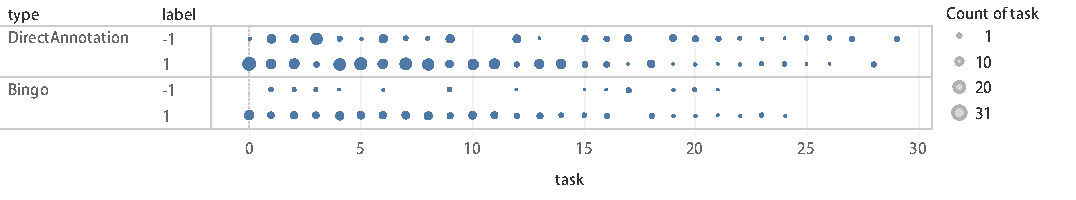
\includegraphics[width=\linewidth]{figures/label.pdf}
\caption{Labeling collected with game \emph{DirectAnnotation} and \emph{Bingo}.}
\label{fig:direct-label}
\end{figure*}


\begin{figure*}[t]
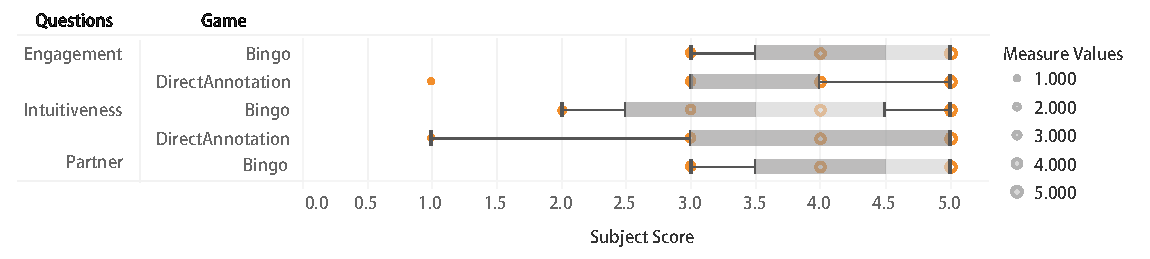
\includegraphics[width=\linewidth]{figures/interview.pdf}
\caption{Labeling collected with game \emph{DirectAnnotation}.}
\label{fig:interview}
\end{figure*}

\subsection{Context} 
While our games can be generally used for text classification tasks, we ask the workers to perform sentiment analysis on IMDB movie reviews~\cite{alsallakh2014visual} in our experiment. 
We choose such a task because 
(1) movie reviews require minimal domain-specific knowledge. Most people could read and understand it, which makes it an ideal source for being a crowdsourced task, and
(2) the sentiment analysis for movie reviews is difficult, as many reviews contain humorous or ironic elements that make the movie sentiment orientation tricky to identify. The broadly distributed difficulty leads to more interesting variations in the collected data.

In our task, we manually selected thirty reviews, 17 positive ones and 13 negative ones.
We manually coded the difficulty of each movie review based on our empirical understanding, and made sure the difficulty is evenly distributed. 


\section{Data Collection} 
\label{sec:analysis}

\subsection{Recorded data} 
The set of features that can be collected from different games are presented below. 

\begin{center}
\begin{tabular}{|c|cccc|}
\hline
Data  & Ann. & Bin. &  H.Add  &   H.Sub   \\
 \hline
Labels-full & \textbullet & \textbullet & \textbullet & \textbullet  \\
Labels-verify &  & $\circ$ & \textbullet & \textbullet  \\
Features-init & \textbullet & \textbullet & \textbullet & \textbullet  \\
Features-rank &  & \textbullet & \textbullet & \textbullet  \\
Features-refine &  &  &  & \textbullet  \\
Features-verify &  & \textbullet & \textbullet & \textbullet  \\\hline
\end{tabular}
\label{table:dataCollect}
\end{center}

{\emph{Labels-full} refers to whether we can extract sentiment label from the game, \emph{labels-verify} refers to whether the game supports different players to verify their label result, \emph{feature-init} refers to whether the game obtains features provided by the gamer, \emph{feature-rank} refers to whether obtained features are ranked, \emph{feature-refine} refers to whether the player can refine initially collected feature, and \emph{feature-verify} refers to whether features are verified though multiple players.}

\subsection{Exit Survey}
Besides the log data, we have also asked the workers to fill in a post-task questionnare (exit survey). We asked them to evaluate the engagement (``\emph{The game is engaging}'') and intuitiveness (``\emph{I could complete the game easily}'') of the game they played. 
Additionally, as all the games except for the benchmark, \emph{Direction-Annotation}, are paired games, we also asked them to evaluate the social impact by scoring ``\emph{I care about my partner's performance greatly}''.

\section{Results}

Due to time limit, we have only deployed game \emph{Bingo} and baseline \emph{DirectAnnotation} so far. As a result, our evaluation focuses on analyzing players' performance in \emph{Bingo} instead of performing inter-game feature comparison. We leave rest proposed experiments as part of future work.

\subsection{Label Accuracy}

Figure~\ref{fig:direct-label} shows labels collected from the baseline game \emph{DirectAnnotation} and \emph{Bingo}. From the figure we noticed that labels corrected through direct annotation have a higher chance of being wrong. For example, document 1, 2, and 6 have nearly half labels wrong in game \emph{DirectAnnotation} while most players made it correct in \emph{Bingo}. We reviewed these cases and found out that these documents are negative reviews containing ironic elements. In these cases, \emph{DirectAnnotation} players receives no feedback from other players and tend to misunderstood the document; in contrast, although players have same document access as before in \emph{Bingo}, the pair-wise agreement module lets them review and carefully think about their decision more carefully, so that they tend to make less mistakes for such tricky documents.


\begin{figure}[t]
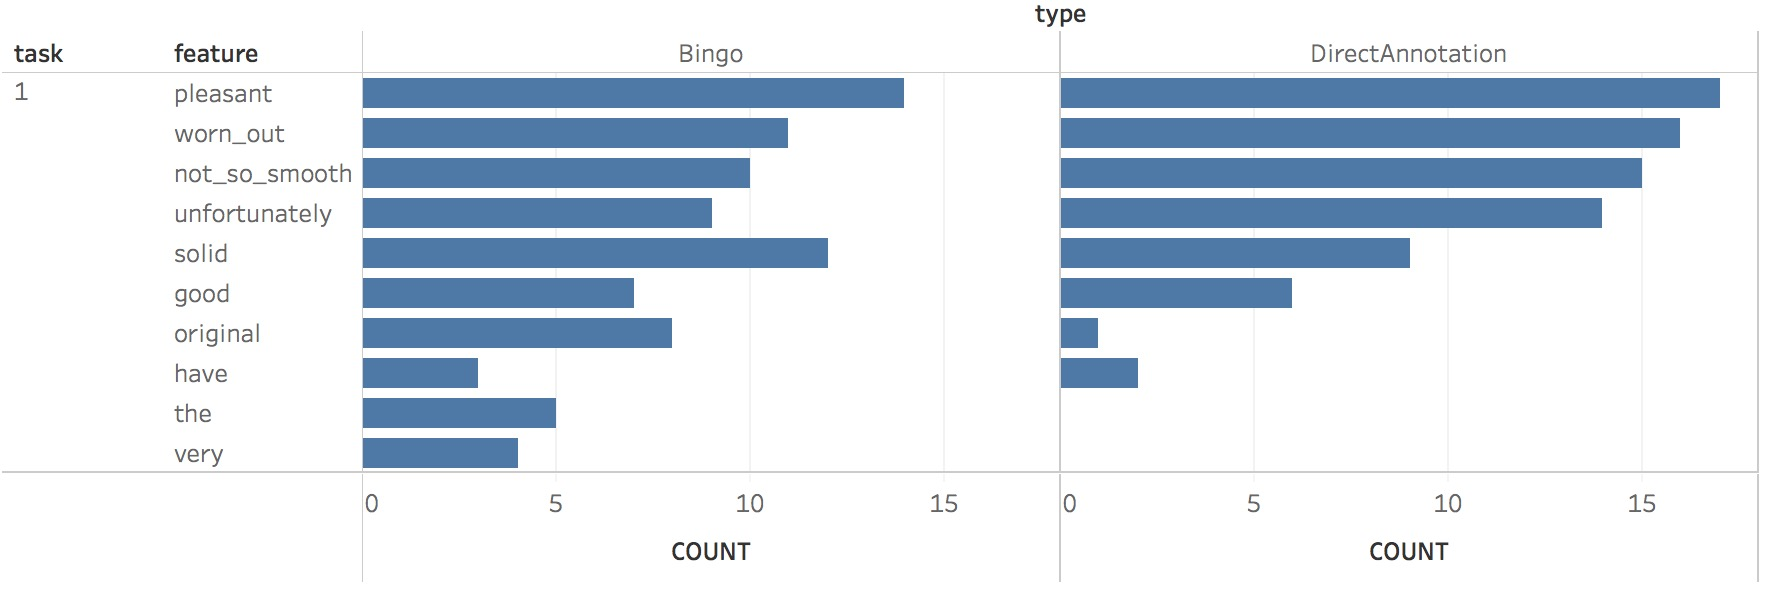
\includegraphics[width=\linewidth]{figures/feature-doc-1}
\caption{Features collected for document 1 with game \emph{DirectAnnotation} and \emph{Bingo}.}
\label{fig:interview}
\end{figure}

\begin{figure}[t]
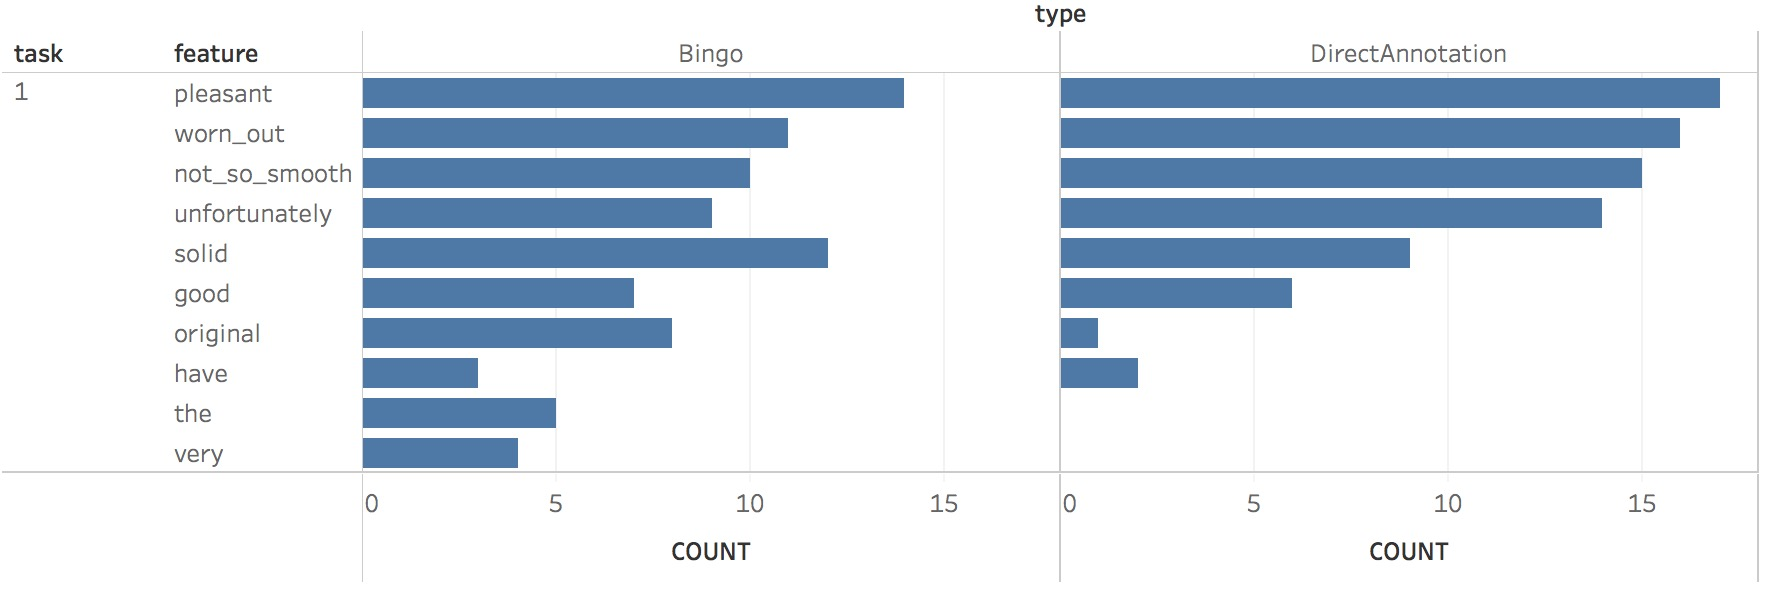
\includegraphics[width=\linewidth]{figures/feature-doc-2}
\caption{Features collected for document 2 with game \emph{DirectAnnotation} and \emph{Bingo}.}
\label{fig:interview}
\end{figure}

\subsection{Features}




\subsection{Engagement}
 Our survey about engagement and intuitiveness of the games is shown in Figure~\ref{fig:interview}. In general, players find game \emph{Bingo} more 

\section{Conclusion}

\section{Discussion}
In our study, we present the problem of mapping human understanding of a machine learning problem onto a constrained model (bag-of-words) using crowdsourcing games. We designed several systems to evaulate how we can effectively learn human understanding. Our results show that such methods of learning latent human features is promising and that further examination of such systems could lead to better design of iML systems.

We also evaluate the effectiveness of each presented game model and classes of games (competitive versus collaborative) and look at their effect on collected features. The goal here is to examine how different tasks posed may affect the final outcome of human judgment. This presents interesting perspectives in how to design iML systems to elicit specific kinds of feedback from humans.

We think that this serves as a good pilot on further developing models of ``human features'' and is useful in future work on designing iML systems.

\section{Future Work}
Our game designs represent a fairly limited subset of games possible with text based analysis. In this paper we examine a relatively simplistic machine model for text to evaulate the feasibility of game based models. We imagine that with more complex models like n-gram or grammar based features, different designs for games can potentially be utilized and tested.

Another potential interesting extension would be a more in-depth study of the incentive structures presented in the games that we have discussed. While our models of incentives are designed to prevent several base cases of degenerative play (i.e. plays where one side being passive leading to decent returns compared to being actively involved), the incentive models have not been extensively tested. We think that it is possible to derive better models that incentivize competitive behavior or collaborative behavior with more in-depth analysis of the game structure presented in our paper.

% REFERENCES FORMAT
% References must be the same font size as other body text.
\bibliographystyle{SIGCHI-Reference-Format}
\bibliography{sample}

\end{document}

%%% Local Variables:
%%% mode: latex
%%% TeX-master: t
%%% End:
